\let\lesson\undefined
\newcommand{\lesson}{\phantomlesson{Bài 9.}}
\setcounter{section}{2}
\section{Bài tập trắc nghiệm}
\begin{enumerate}[label=\bfseries Câu \arabic*:]
	\item \mkstar{1}\\
	{Một vật ném xiên có quỹ đạo như hình vẽ. Tầm bay xa của vật là khoảng cách giữa
		\begin{center}
			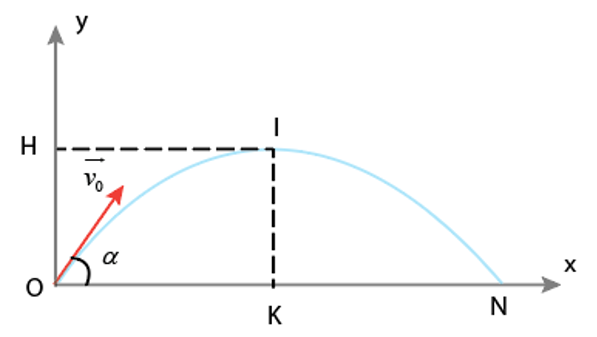
\includegraphics[width=0.4\linewidth]{../figs/VN10-2022-PH-TP013-P-1}
		\end{center}
	\begin{mcq}
		\item điểm ném và điểm cao nhất của quỹ đạo.
		\item điểm cao nhất của quỹ đạo và điểm rơi.
		\item điểm cao nhất của quỹ đạo và điểm có gia tốc bằng 0.
		\item điểm ném và điểm rơi trên mặt đất.
	\end{mcq}
}
\hideall{
\textbf{Đáp án: D.}
}

\item \mkstar{1}\\
{Một quả tạ được ném từ độ cao $h$ sao cho vận tốc ban đầu $\overrightarrow{v_0}$ hợp với phương ngang một góc $\alpha$. Tầm xa của quả tạ phụ thuộc vào
	\begin{mcq}(2)
		\item góc ném $\alpha$ và vận tốc ban đầu $v_0$.
		\item lực cản của không khí.
		\item độ cao $h$.
		\item tất cả các yếu tố trên.
	\end{mcq}

}
\hideall{
\textbf{Đáp án: D.}
}

\item \mkstar{1}\\
{Một vật ném xiên có quỹ đạo như hình vẽ. Tầm cao của vật ném xiên là đoạn
\begin{center}
	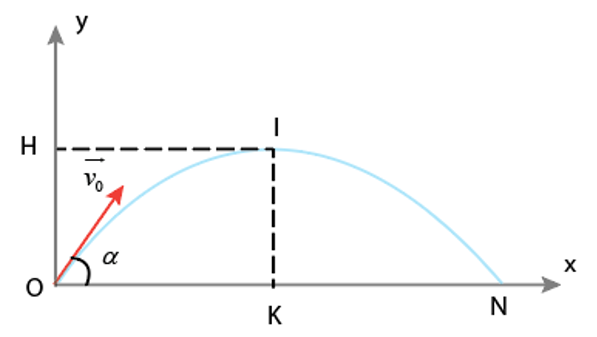
\includegraphics[width=0.4\linewidth]{../figs/VN10-2022-PH-TP013-P-1}
\end{center}
\begin{mcq}(4)
	\item IK.
	\item OI.
	\item OK.
	\item NO
\end{mcq}
}
\hideall{
\textbf{Đáp án: A.}
}

\item \mkstar{2}\\
{Trong hình vẽ sau, gia tốc của vật tại đỉnh I có
	\begin{center}
		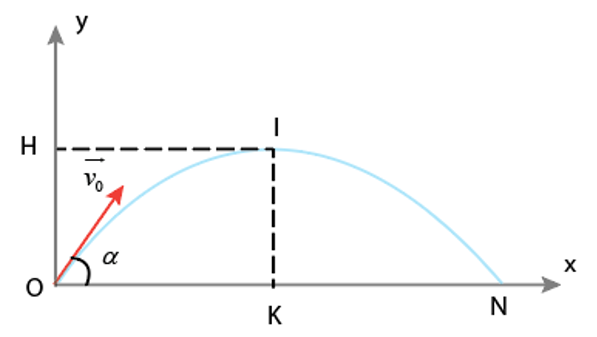
\includegraphics[width=0.4\linewidth]{../figs/VN10-2022-PH-TP013-P-2}
	\end{center}
\begin{mcq}(2)
	\item hướng ngang theo chiều từ H đến I.
	\item hướng ngang theo chiều từ I đến H.
	\item hướng thẳng đứng xuống dưới.
	\item hướng thẳng đứng lên trên.
\end{mcq}
}
\hideall{
\textbf{Đáp án: C.}
}

\item \mkstar{3}\\
{Một vật được ném xiên từ mặt đất lên với vận tốc ban đầu là $v_0 = \SI{10}{\meter/\second}$ theo phương hợp với phương nằm ngang góc $\SI{30}{\degree}$. Lấy $g = \SI{10}{\meter/\second^2}$. Độ cao cực đại và tầm xa mà vật đạt được lần lượt là
	\begin{mcq}(4)
		\item $\SI{1.25}{\meter}$; $\SI{8.66}{\meter}$.
		\item $\SI{8.66}{\meter}$; $\SI{1.25}{\meter}$.
		\item $\SI{1.25}{\meter}$; $\SI{22.5}{\meter}$.
		\item $\SI{22.5}{\meter}$; $\SI{8.66}{\meter}$.
	\end{mcq}

}
\hideall{
\textbf{Đáp án: A.}
}

\item \mkstar{3}\\
{Một vật được ném lên từ mặt đất theo phương xiên góc hợp với phương ngang một góc $\alpha =\SI{45}{\degree}$, với vận tốc ban đầu là $\SI{5}{\meter/\second}$. Bỏ qua mọi lực cản. Lấy $g = \SI{10}{\meter/\second^2}$. Độ cao cực đại của vật là
\begin{mcq}(4)
	\item $\SI{0.25}{\meter}$.
	\item $\SI{0.5}{\meter}$.
	\item $\SI{0.625}{\meter}$.
	\item $\SI{1.25}{\meter}$.
\end{mcq}
}
\hideall{
\textbf{Đáp án: C.}
}

\item  \mkstar{3}\\
{Một vật được ném với vận tốc $\SI{12}{\meter/\second}$ từ mặt đất với góc ném $\alpha=\SI{30}{\degree}$ so với mặt phẳng nằm ngang. Lấy $g = \SI{10}{\meter/\second^2}$. Hòn đá rơi đến đất cách chỗ ném theo phương ngang một khoảng $\SI{200}{\meter}$. Thời gian hòn đá rơi là
\begin{mcq}(4)
	\item $\SI{24.5}{\second}$.
	\item $\SI{19.2}{\second}$.
	\item $\SI{14.6}{\second}$.
	\item $\SI{32.8}{\second}$.
\end{mcq}
}
\hideall{
\textbf{Đáp án: B.}
}

\item \mkstar{3}\\
{Một vật được ném lên từ mặt đất theo phương xiên góc hợp với phương ngang một góc $\alpha$. Khi lên đến độ cao cực đại cách mặt đất $\SI{15}{\meter}$ thì vận tốc bằng một nửa vận tốc ban đầu. Lấy $g =\SI{10}{\meter/\second^2}$. Tính độ lớn vận tốc ban đầu.
	\begin{mcq}(4)
		\item $\SI{18}{\meter/\second}$.
		\item $\SI{20}{\meter/\second}$.
		\item $\SI{15}{\meter/\second}$.
		\item $\SI{25}{\meter/\second}$.
	\end{mcq}

}
\hideall{
\textbf{Đáp án: B.}
}

\item \mkstar{4}\\
{Từ độ cao $\SI{7.5}{\meter}$ người ta ném một quả cầu với vận tốc ban đầu $\SI{10}{\meter/\second}$, ném xiên góc $\SI{45}{\degree}$ so với phương ngang. Vật chạm đất tại vị trí cách vị trí ban đầu
	\begin{mcq}(4)
		\item $\SI{5}{\meter}$.
		\item $\SI{15}{\meter}$.
		\item $\SI{9}{\meter}$.
		\item $\SI{18}{\meter}$.
	\end{mcq}

}
\hideall{
\textbf{Đáp án: B.}
}

\item \mkstar{4}\\
{Từ một đỉnh tháp cao $\SI{12}{\meter}$ so với mặt đất, người ta ném một hòn đá với vận tốc ban đầu $v_0=\SI{15}{\meter/\second}$, theo phương hợp với phương nằm ngang một góc $\alpha=\SI{45}{\degree}$. Khi chạm đất, hòn đá có vận tốc bằng bao nhiêu? Lấy $g = \SI{9.8}{\meter/\second^2}$.
\begin{mcq}(4)
	\item $\SI{18.6}{\meter/\second}$.
	\item $\SI{24.2}{\meter/\second}$.
	\item $\SI{28.8}{\meter/\second}$.
	\item $\SI{21.4}{\meter/\second}$.
\end{mcq}
}
\hideall{
\textbf{Đáp án: D.}
}
\end{enumerate}
\section{Bài tập tự luận}
\begin{enumerate}[label=\bfseries Bài \arabic*:]
	\item \mkstar{3}
	
	
	{Một vật ném xiên góc $45^\circ$ từ mặt đất và rơi cách đó $\SI{30}{m}$. Tính vận tốc khi ném, lấy $g=\SI{10}{m/s}^2$.
	}
	
	\hideall
	{	
		
		Vận tốc khi bị ném
		
		$$L = \dfrac{v^2_0 \sin 2\alpha}{g} = 30 \Rightarrow v_0 = \xsi{10\sqrt 3}{m/s}.$$
	}
	
	
	\item \mkstar{3}
	
	
	{Vật được ném xiên góc $60^\circ$ với vận tốc $\SI{30}{m/s}$, lấy $g=\SI{10}{m/s}^2$, tính tầm xa và độ cao cực đại vật đạt được.
	}
	
	\hideall
	{	
		Tầm xa của vật
		
		$$L = \dfrac{v^2_0 \sin 2\alpha}{g} = \SI{77,94}{m}.$$
		
		Độ cao cực đại
		
		$$H = \dfrac{v^2_0\sin^2 2\alpha}{2g} = \SI{33,75}{m}.$$
		
	}
	\item \mkstar{3}
	
	
	
	{Ném xiên góc $45^\circ$ một vật với vận tốc $\SI{25}{m/s}$. Lấy $g=\SI{10}{m/s}^2$, tính vận tốc của vật sau khi ném $\SI{1,2}{s}$.
	}
	
	\hideall
	{	
		Ta có:
		
		$$\begin{cases}
			v_\text{x} = v_0 \cos \alpha = \SI{17,677}{m/s}.\\
			v_\text{y} = v_0 \sin \alpha - gt = \SI{5,677}{m/s}.
		\end{cases}$$
		
		Vận tốc của vật
		
		$$v = \sqrt{v^2_\text{x} + v^2_\text{y}} = \SI{18,6}{m/s}.$$
		
	}
	\item \mkstar{3}
	
	
	
	{Từ mặt đất một vật được ném xiên với phương ngang một góc $\alpha = 45^\circ$ với vận tốc ban đầu là $\SI{20}{m/s}$. Lấy $g=\SI{10}{m/s}^2$. Viết phương trình chuyển động của vật và độ cao mà vật có thể lên tới.
	}
	
	\hideall
	{	
		
		\begin{center}
			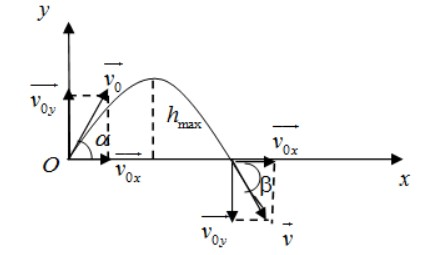
\includegraphics[scale=1.2]{../figs/VN10-2021-PH-TP014-2.jpg}
		\end{center}
		
		Thời điểm ban đầu
		
		Chiếu lên trục Ox có $x_0 = 0$
		
		$$v_{0\text{x}} = v_0 \cos \alpha = \xsi{10\sqrt 2}{m/s}.$$
		
		Chiếu lên trục Oy có $y_0 = 0$
		
		$$v_{0\text{y}} = v_0 \sin \alpha = \xsi{10\sqrt 2}{m/s}.$$	
		
		Xét tại thời điểm $t$ có
		
		$$a_\text{x} = 0; a_\text{y} = -g.$$
		
		Chiếu lên trục Ox ta có:
		
		$$v_\text{x} = \xsi{10\sqrt 2}{m/s}; x = 10\sqrt 2 t.$$
		
		Chiếu lên trục Oy ta có:
		
		$$v_\text{y} = 10\sqrt 2 - 10t; y = 10\sqrt 2 t - 5t^2.$$
		
		$$\Rightarrow y = x - \dfrac{x^2}{40}.$$
		
		Vậy quỹ đạo của vật là một parabol.
		
		Khi lên đến độ cao cực đại thì
		
		$$v_\text{y} = 0 \Rightarrow 10\sqrt 2 - 10t =0 \Rightarrow t = \xsi{\sqrt 2}{s}$$
		
		$$\Rightarrow h_\text{max} = y = \SI{10}{m}.$$
	}
\item \mkstar{4}


{Từ A (độ cao AC = $H$ = $\SI{3,6}{m}$) người ta thả một vật rơi tự do, cùng lúc đó từ B cách C đoạn BC = $L$ = $H$ người ta ném một vật khác với vận tốc ban đầu $v_0$ hợp với phương ngang góc $\alpha$. Tính $\alpha$ và $v_0$ để hai vật gặp được nhau khi vật A qua vị trí bằng 1 nửa độ cao ban đầu. Lấy gia tốc rơi tự do $g=\SI{10}{\meter/\second^2}$.
	
	\begin{center}
		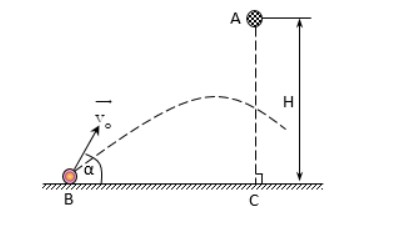
\includegraphics[scale=1]{../figs/VN10-2021-PH-TP014-1.jpg}
	\end{center} 
}

\hideall
{	Chọn gốc toạ độ tại C, trục $Oy$ thẳng đứng hướng lên, trục $Ox$ hướng từ B sang C.
	
	Phương trình vật thả rơi (vật I):
	
	$$x_1 = 0; y_1 = H -\text{0,5}gt^2.$$
	
	Phương trình vật II:
	
	$$\begin{cases}
		x_2 = L  - (v_0 \cos \alpha)t = H - (v_0\cos \alpha)t.\\
		y_2 = (v_0\sin \alpha) t - \text{0,5}gt^2.
	\end{cases}$$
	
	Để hai vật gặp nhau $x_1 = x_2$ và $y_1 = y_2$
	
	$$\begin{cases}
		(v_0\cos \alpha) t = H.\\
		(v_0 \sin \alpha)t = H.
	\end{cases} \Rightarrow \tan \alpha = 1 \Rightarrow \alpha = \SI{45}{\degree}$$
	
	Nhân 2 vế của hệ phương trình trên với nhau ta được
	$$v^2_0\cdot\dfrac{\sin2\alpha}{2}\cdot t^2=H^2 \Rightarrow v_0=\dfrac{H\sqrt{2}}{t\sqrt{\sin2\alpha}}$$
	
	Mà hai vật gặp nhau tại vị trí $y_1=\dfrac{H}{2}\Rightarrow t=\sqrt{\dfrac{H}{g}}\Rightarrow v_0=\sqrt{\dfrac{2Hg}{\sin 2\alpha}} = \xsi{6\sqrt{2}}{m/s}.$
}
\end{enumerate}
